% !TeX spellcheck = pl_PL

\rozdzial

%%%%%%%%%%%%%%%%%%%%%%%%%%%%%%%%%%%%%%%%%%%%%%%%%%%%%%%%%%%%%%%%%%%%%%%
\section{Interfejs wejściowy PS/2}
\label{ps2}


PS/2 jest prostym interfejsem szeregowym synchronicznym wykorzystywanym w~myszach i klawiaturach komputerowych. Aktualnie jest wypierany przez standard USB, który jest znaczenie trudniejszy do realizacji w układzie FPGA. Istnieją konwertery pozwalające podłączyć urządzenia wejściowe USB do portu PS/2, dlatego wybór tego standardu nadal wydaje się uzasadniony.


Interfejs posiada linie danych i zegara. Obie są dwukierunkowe i pracują w~standardzie~5V, dlatego nie jest możliwe bezpośrednie podłączenie ich do układu FPGA. Rysunek \ref{PS2Electrical} przedstawia schemat elektryczny zastosowany do podpięcia jednej linii w standardzie PS/2. Obniżenie napięcia wejściowego z 5V na 3,3V odbywa się przez dzielnik rezystorowy, natomiast wyjście realizowane jest przy pomocy tranzystora NPN ściągającego linię danych do masy. Gdy linia nie jest aktywna rezystor ,,pull-up'' utrzymuje stan wysoki.


\begin{figure}[h]	
	\centering
	\obrazpng{0 0 1054 861}{8cm}{obrazki/PS2Electrical.png}
	\caption{ Schemat elektryczny podłączenia jednej linii w standardzie PS/2. }
	\label{PS2Electrical}
\end{figure}

\begin{figure}[htb]
	\centering
	\begin{subfigure}[b]{6cm}
		\obrazpng{0 0 1471 893}{6cm}{obrazki/PS2Dev2Host.png}
		\caption{ Z urządzenia (FPGA nie uczestniczy aktywnie) }
	\end{subfigure}
	~
	\begin{subfigure}[b]{7.5cm}
		\obrazpng{0 0 1471 893}{7.5cm}{obrazki/PS2Host2Dev.png}
		\caption{ Z FPGA (HOST) do urządzenia (DEVICE) }
	\end{subfigure}
	\caption{ Przebiegi sygnałów wysyłania i odbierania bajtu \cite{PS2eng}. }
	\label{PS2Signals}
\end{figure}

Przebiegi sygnałów PS/2 przedstawia rysunek \ref{PS2Signals}. Odbiór danych z urządzenia nie jest trudny -- wymaga tylko rejestru przesuwnego wyzwalanego narastającym zboczem zegara oraz logiki wykrywającej koniec transmisji. Transmisja w drugą stronę jest bardziej złożona i wymaga odpowiedniej maszyny stanów. Oba zadania są realizowane przez wykonany moduł. Zadaniem interpretacji danych zawartych w transmitowanych pakietach zajmuje się biblioteka napisana dla PicoBlaze'a.

\subsection{Struktura modułu}

Interfejs PS/2 nie jest możliwy do realizacji w całości przez oprogramowanie uruchamiane na procesorze PicoBlaze ze względu na restrykcje czasowe i sygnał zegara generowany przez urządzenie zewnętrze. Z tego powodu konieczne było zaimplementowanie odpowiedniego modułu w Verilog'u. Moduł do obsługi PS/2 został wykonany w dwóch wariantach:
\begin{itemize}
	\item Wariant uproszczony pozwala na obsługuję tylko danych odbieranych przez PS/2. Taka redukcja modułu znacznie zmniejsza ilość potrzebnych zasobów FPGA i~wystarcza do obsługi klawiatury w podstawowym zakresie, co w tym systemie jest wystarczające. Uproszony schemat tego wariantu znajduje się na rysunku \ref{ps2input_flow}.
	\item Wariant pełen zapewnia dwukierunkową transmisję danych przez PS/2. Takie rozwiązanie jest konieczne do obsługi myszy, która po podłączeniu musi zostać skonfigurowana. Uproszony schemat tego wariantu znajduje się na rysunku \ref{ps2inputOutput}.
\end{itemize}


Sygnał zegara PS/2 generowany jest przez urządzenie i ma on częstotliwość od 10 do 16 KHz. Dane wejściowe odczytywane są przy zboczu narastającym tego zegara, dlatego ważne jest, aby sygnał nie zawierał zakłóceń -- każde nieoczekiwane dodatkowe zbocze powoduję uszkodzenie danych wejściowych. Został zaimplementowany filtr, który redukuje zakłócenia. Po zboczu opadającym sygnał musi pozostać stabilny przez określony czas zanim zostanie wystawiony na wyjście filtra. Zbocze narastające przekazywane jest natychmiast na wyjście filtra, aby zredukować czas od pojawiania się zbocza do spróbkowania sygnału danych. Ten filtr zapewnia filtrację tylko przy zmianie stanów. W czasie przeprowadzonych doświadczeń tylko tego typu zakłócenia zostały zaobserwowane.

\begin{figure}[htb]
	\centering
	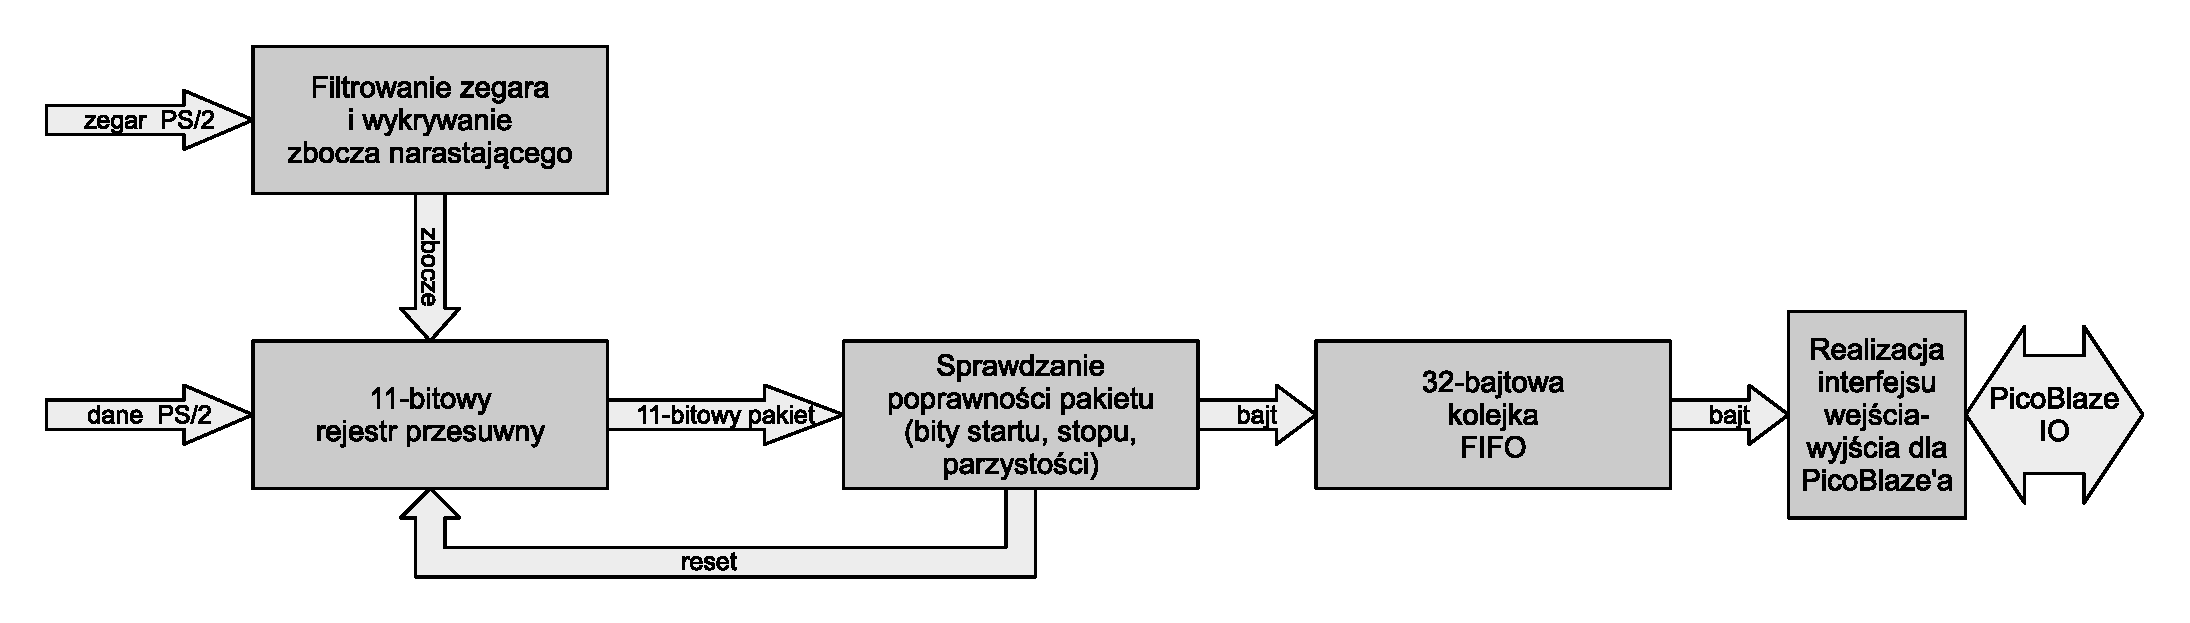
\includegraphics[width=16cm]{obrazki/ps2input_flow.eps}
	\caption{Uproszczony schemat blokowy modułu PS/2 tylko do odbioru danych.}
	\label{ps2input_flow}
\end{figure}

Tak przefiltrowany sygnał zegara wyzwala przesunięcie 11-bitowego rejestru przesuwnego i wsunięcie do niego aktualnego bitu danych. Jeżeli cały rejestr zawiera poprawy pakiet danych (istnieje bit startu i stopu), to rejestr jest czyszczony, a~odczytany bajt wędruje dalej do kolejki FIFO.

Oprogramowanie nie musi natychmiast odczytać danych wejściowych, dlatego konieczna jest kolejka FIFO, aby nie dopuścić do utraty danych. Jest ona rozmiaru 32 bajtów. Przy najgorszych warunkach wymusza to konieczność sprawdzania danych wejściowych przez oprogramowanie co 20ms. Dane wyciągane są z kolejki przez interfejs procesora PicoBlaze opisany dokładniej w rozdziale \ref{Interfejs_dla_procesora_PicoBlaze}.


\begin{sidewaysfigure}[p]
	\centering
	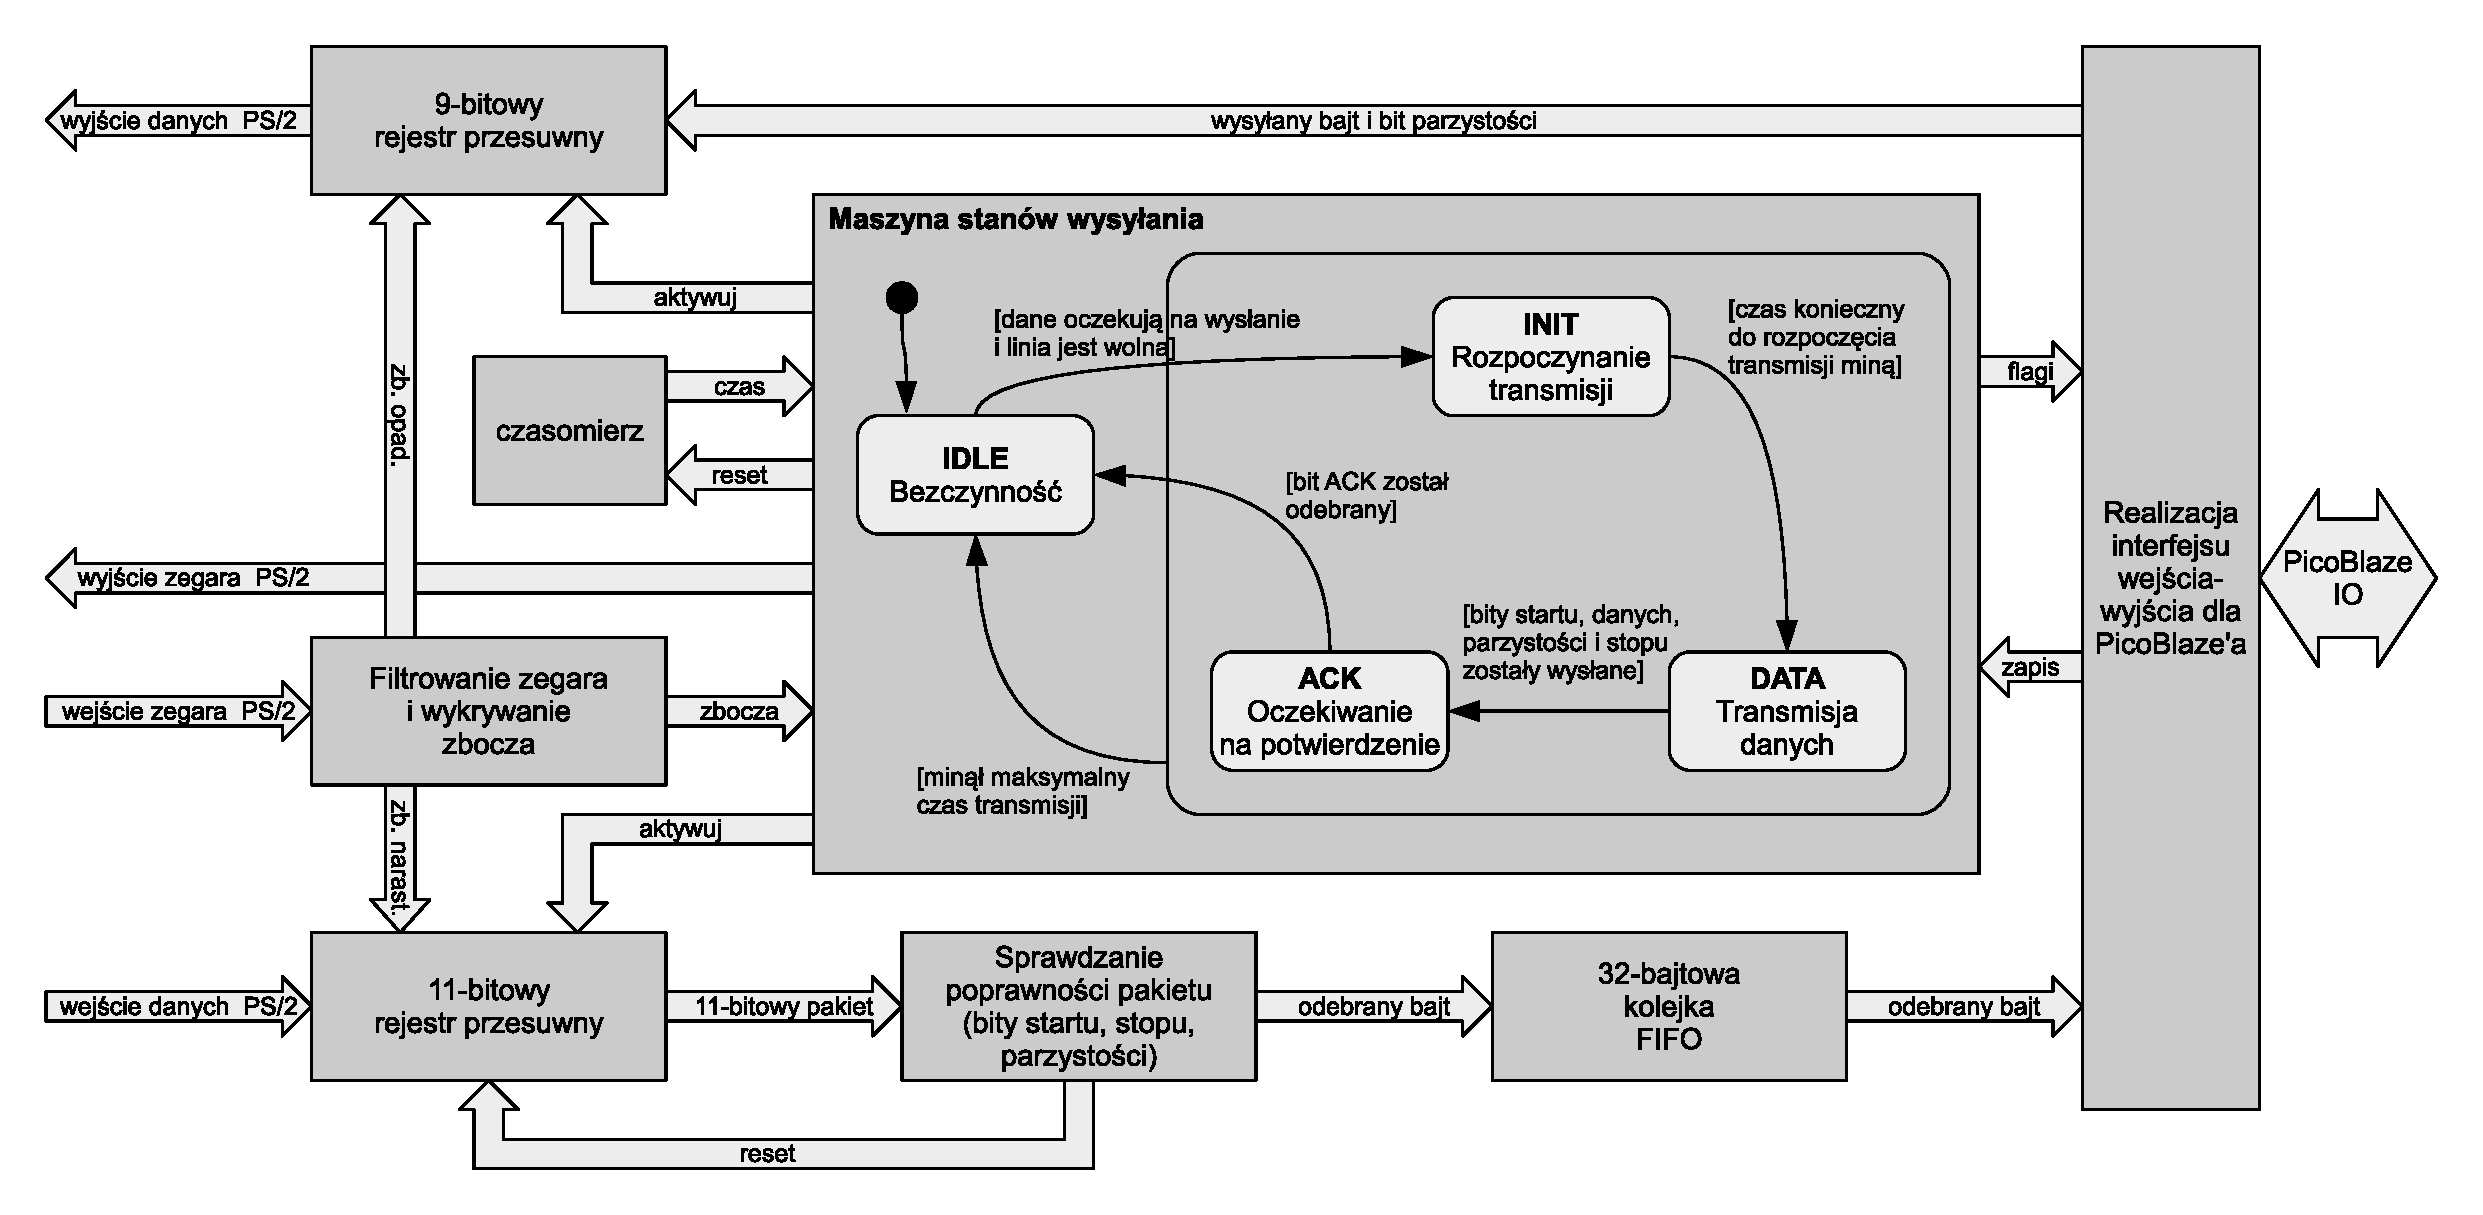
\includegraphics[width=22cm]{obrazki/ps2inputOutput.eps}
	\caption{Uproszczony schemat blokowy modułu PS/2 z możliwością odbioru i wysyłania danych.}
	\label{ps2inputOutput}
\end{sidewaysfigure}


Pełen wariant modułu został wyposażony w dodatkowe elementy wysyłające dane przez PS/2, które można zobaczyć na rysunku \ref{ps2inputOutput}. Sercem części wysyłającej jest maszyna stanów, która korzysta z czasomierza i rejestru przesuwnego podającego bity na wyjście danych PS/2. Zdefiniowane są cztery stany:
\begin{itemize}
	\item \textbf{,,IDLE''} -- W tym stanie aktywny jest 11-bitowy rejestr przesuwny wejścia, więc odbiór danych jest możliwi. W każdym innym stanie wejście jest zablokowane. Przejście do kolejnego stanu następuje, gdy programista wpisał wartość do rejestru danych i linia PS/2 jest aktualnie wolna.
	\item \textbf{,,INIT''} -- Stan wyjścia zegara jest niski przez co najmniej 100$\mu$s, co jest konieczne do poprawnego rozpoczęcia transmisji. Po tym czasie następuje przejście do kolejnego stanu.
	\item \textbf{,,DATA''} -- 9-bitowy rejestr przesuwny wyjścia jest aktywny, więc na wyjście PS/2 trafiają kolejne bity. Gdy wszystkie zostaną wysłane, następuje przejście do kolejnego stanu.
	\item \textbf{,,ACK''} -- Urządzenie po otrzymaniu danych musi wysłać jeden bit potwierdzający poprawny odbiór. W tym stanie odbywa się oczekiwanie i odczyt tego bitu. Po odczycie następuje przejście do stanu ,,IDLE''.
\end{itemize}

Transmisja sterowana jest zegarem generowanym przez urządzenie. Może zaistnieć sytuacja, kiedy sygnał nie jest generowany poprawnie, np. urządzenie zostało odpięte. W~takiej sytuacji maszyna stanów zatrzyma się w stanie innym niż ,,IDLE'' nawet po usunięciu problemu, np. po podłączeniu urządzenia. Aby dalsza komunikacja była możliwa, zaimplementowano przejście do stanu ,,IDLE'' po przekroczeniu maksymalnego czasu transmisji. Informacja o takiej sytuacji dostępna jest dla programisty przez odpowiednią flagę.

\subsection{Interfejs dla procesora PicoBlaze}
\label{Interfejs_dla_procesora_PicoBlaze}

Moduł posiada dwa rejestry wejścia-wyjścia. Adres bazowy jest definiowalny przez użytkownika w kodzie Verilog i może być całkowicie dowolny -- nie ma restrykcji co do wyrównania lub zakresu. Taka elastyczność pozwala uniknąć ewentualnych konfliktów z~innymi urządzeniami podpiętymi do PicoBlaze'a oraz dodać wiele instancji tego modułu. Adresy rejestrów w poniższym opisie są podane względem tego adresu bazowego.


\begin{table}[h]
	\begin{center}
	{\footnotesize
		\begin{tabular}{|l|l|l|l|l|l|l|l|}
			\hline
			\multicolumn{8}{|l|}{ \textbf{PS2D - PS/2 Data Register} } \\
			\hline
			\multicolumn{3}{|l}{ Adres: 0x00 } & \multicolumn{5}{l|}{ Odczyt-zapis } \\
			\hline
			\hline bit 7 & bit 6 & bit 5 & bit 4 & bit 3 & bit 2 & bit 1 & bit 0 \\				
			\hline \textbf{PS2D7} & \textbf{PS2D6} & \textbf{PS2D5} & \textbf{PS2D4} & \textbf{PS2D3} & \textbf{PS2D2} & \textbf{PS2D1} & \textbf{PS2D0} \\				
			\hline
		\end{tabular}}
		\caption{ Rejestr PS2D }
		\label{tab:regPS2D}
	\end{center}
\end{table}


Rejestr \textbf{PS2D} służy do wysyłania i odbierania danych przez PS/2. Gdy flaga PS2DR jest ustawiona, należy odczytać ten rejestr w celu pobrania bajtu odczytanego z interfejsu PS/2. W celu wysłania bajtu należy zapisać zadaną wartość do tego rejestru i zaczekać, aż flaga PS2B zostanie wyczyszczona.


\begin{table}[h]
	\begin{center}
	{\footnotesize
		\begin{tabular}{|l|l|l|l|l|l|l|l|}
			\hline
			\multicolumn{8}{|l|}{ \textbf{PS2F - PS/2 Flags Register} } \\
			\hline
			\multicolumn{3}{|l}{ Adres: 0x01 } & \multicolumn{5}{l|}{ Tylko do odczytu } \\
			\hline
			\hline bit 7~~~~ & bit 6~~~~ & bit 5~~~~ & bit 4~~~~ & bit 3~~~~ & bit 2~~~~ & bit 1~~~~ & bit 0~~~~ \\				
			\hline - & - & -& - & \textbf{PS2TO} & \textbf{PS2ACK} & \textbf{PS2B} & \textbf{PS2DR} \\				
			\hline
		\end{tabular}}
		\caption{ Rejestr PS2F }
		\label{tab:regPS2F}
	\end{center}
\end{table}


Rejestr \textbf{PS2F} posiada trzy flagi tylko do odczytu:
\begin{itemize}
	\item Flaga \textbf{PS2DR (PS/2 Data Ready)} zostaje ustawiona, gdy moduł odebrał bajt danych. Oznacza to, że należy odczytać rejestr PS2D. Po odczytaniu wszystkich danych flaga zostanie automatycznie wyczyszczona.
	\item Flaga \textbf{PS2B (PS/2 Busy)} zostaje ustawiona w momencie zapisu do PS2D. Oznacza to, że wysyłanie danych przez port PS/2 rozpoczęło się. Gdy transmisja zakończy się (sukcesem lub porażką), flaga zostanie automatycznie wyczyszczona.
	\item Flaga \textbf{PS2ACK (PS/2 Ack)} jest ustawiona, gdy urządzenie potwierdziło odbiór ostatniego wysłanego bajta, wyczyszczona w przeciwnym wypadku.
	\item Flaga \textbf{PS2TO (PS/2 Timeout)} jest ustawiona, gdy ostatni bajt nie został wysłany, ponieważ urządzenie nie rozpoczęło odbierania danych w określonym czasie (co najmniej 10ms).
\end{itemize}


Wersja modułu umożliwiająca tylko odczyt danych posiada PS2D w trybie tylko do odczytu oraz nie posiada flag PS2B, PS2ACK i PS2TO. Wszystkie nie używane bity rejestrów mają niezdefiniowaną wartość przy odczycie. Wartość zapisana do nich nie ma znaczenia.

\subsection{Biblioteka do obsługi urządzeń PS/2}

Komunikacja przez PS/2 realizowana jest przez przygotowaną do tego celu bibliotekę. Dzięki temu nie jest koniczne bezpośrednie operowanie na rejestrach. Biblioteka podzielona jest na trzy pliki. Wybrane pliki należy dodać do głównego pliku programu dyrektywą ,,INCLUDE''.

\begin{itemize}
	\item  \textbf{,,ps2\_keyboard.psm''} -- część biblioteki odpowiedzialna za obsługę klawiatury. Należy ją dodać, gdy do systemu będzie podłączana klawiatura. Przed dodaniem należy zdefiniować stałe (dyrektywa ,,CONSTANT'') o nazwie PS2\_KEYBOARD\_PS2D i PS2\_KEYBOARD\_PS2F, które określają adresy rejestrów do obsługi portu klawiatury.
	
	\item  \textbf{,,ps2\_mouse.psm''} -- część biblioteki odpowiedzialna za obsługę myszy. Należy ją dodać, gdy do systemu będzie podłączana mysz. Przed dodaniem należy zdefiniować stałe (dyrektywa ,,CONSTANT'') o nazwie PS2\_MOUSE\_PS2D i~PS2\_MOUSE\_PS2F, które określają adresy rejestrów do obsługi portu myszy.
	
	\item  \textbf{,,ps2\_common.psm''} -- kod biblioteki wspólny dla myszy i klawiatury, który należy zawsze dodać do pliku głównego.
\end{itemize}


Biblioteka udostępnia funkcje, które zwracają użytkownikowi gotowe przetworzone dane. Realizuje również detekcję i inicjalizację urządzeń podłączanych do portu. Najważniejszymi funkcjami biblioteki są:

\begin{itemize}
	\item  \textbf{getKeyCode} -- zwraca kod wciśniętego klawisza lub zero jeżeli klawisz nie został wciśnięty od ostatniego wywołania tej funkcji.
	\item  \textbf{getMouseState} -- zwraca przesunięcie w osi X i Y od ostatniego wywołania i stan przycisków myszy.
\end{itemize}

Użytkownik najczęściej nie będzie wywoływał tych funkcji bezpośrednio. Zamiast tego biblioteka GUI opisana w rozdziale~\ref{guilib_section} współpracuje z tą biblioteką.

